\chapter{Stima di parametri}
In questo capitolo vedremo come usare i dati campionari per stimare una media,
una varianza o una proporzione della popolazione. 
Verranno discusse le \textbf{stime puntuali}, ovvero le stime a valore singolo del parametro,
di cui considereremo poi l'errore standard.
Inoltre considereremo gli intervalli di confidenza, che contengono il parametro
con un certo livello di confidenza.

\section{Statistica inferenziale}
La \textbf{statistica inferenziale} ha lo scopo di definire in modo non ambiguo e
quantitativo la plausibilità di un'inferenza.
\paragraph{Plausibilità}
La plausibilità di un'inferenza dipende dal modo con cui è stato selezionato
un campione di $n$ individui della popolazione.
La corretta metodologia di campionamento è la \textbf{scelta casuale}.
\\ Per la casualità del campionamento utilizzo il calcolo delle probabilità.
\\ Quando parleremo di popolazione tratteremo sempre $N$ molto grandi rispetto all'ampiezza del campione. 
Potremmo anche avere a che fare con popolazioni infinite, as esempio quando si parla di processi produttivi.

La \textbf{popolazione} è una V.A. i.i.d. con la stessa legge $F$ non sempre completamente nota.

\subsection{Modello Statistico Parametrico} 
Il modello statistico parametrico è una famiglia di leggi note a meno di uno o
più parametri: $\underline{\theta} \in I \subseteq R^d, d\geq 1$.
\begin{itemize}
    \item Caso discreto: $p(x; \Theta) \quad$ 
    Densità discreta $p(x;\Theta):\mathbb{P}_\Theta (X=x)$
    \item Caso continuo: densità $f(x; \Theta)$
\end{itemize}
\begin{center}
    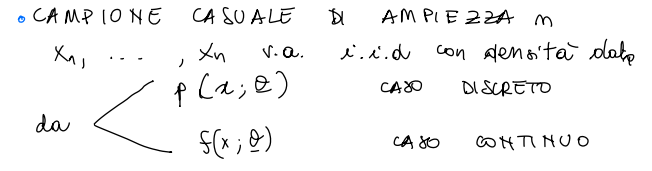
\includegraphics[width=.8\textwidth]{statistica-parametrica.png}
\end{center}
\nb{Attenzione a non confondere le V.A. con le osservazioni:
 \\$X_1, ..., X_n \quad$ sono le Variabili Aleatorie, mentre $x_1, ..., x_n \quad$ sono le Osservazioni
}

\paragraph{Esempi di modelli statistici}
Alcuni esempi di modelli statistici sono:
\begin{itemize}
    \item Modello di Bernoulli
    \item Modello esponenziale
    \item Modello normale
\end{itemize}
\paragraph{Le Statistiche}
Diamo la definizione di statistica:
\definizione{
    Dato $(X_1, ..., X_n)$ campione casuale, si definisce \textbf{Statistica} una
    funzione del campione, ossia una v.a. T della forma
    \[
        T=f(X_1, ..., X_n)
    \]
}
Alcuni esempi di statistica sono:
\begin{itemize}
    \item Media campionaria (v.a.)$\bar{X}_n = \frac{X_1+...+X_n}{n} \quad$ 
    \item Varianza campionaria (v.a.): $S^{2}_n = \frac{1}{n-1} \sum_{i=1}^n(X_i - \bar{X}_n)^2 \quad$
\end{itemize}
\pagebreak

\section{Statistica Parametrica e Stimatori}
Il primo obiettivo della statistica inferenziale è fornire una \emph{stima dei parametri incogniti}.   
\paragraph{Stimatori}

% \textbf{la Stima}, viene usato per predire il valore di un parametro della popolazione.
% particolari statistiche che servono a stimare i parametri incogniti.
% \paragraph*{Stimatori Puntuali} Sono valori singoli che speriamo siano prossimi
% ai parametri stimati.
% \paragraph*{Stimatori intervallari} Meglio noti come \textbf{Intervalli di confidenza},
% in questo caso non rappresentano un singolo valore, ma un intervallo in cui ci
% aspettiamo che il parametro rientri. Ci occupiamo anche di determinare quanta
% confidenza associare a un dato intervallo, cioè quanto possiamo essere sicuro che il parametro
% si trovi in questo intervallo.

Uno \textbf{Stimatore} è una statistica che serve a stimare i parametri incogniti:
\definizione{
    Uno stimatore $T$ si dice \textbf{Non Distorto} o corretto se:
    \[ E_\theta (T) = E_\theta (g(X_1,...,X_n)) = \theta \]
    In cui $E_\theta$ è il valore medio rispetto alla probabilità $P_\theta$.
}
In parole povere uno stimatore il cui valore atteso è uguale al parametro
che si vuole stimare si dice \textbf{corretto} per quel parametro.

Ad esempio, qualunque sia il campione casuale $X_1,...,X_n$, con $\mu = E(X_1)\geq +\infty$:
\begin{center}
    $\bar{X}_n$ è uno stimatore non distorto di $\mu$, quindi $E(\bar{X}_n = \mu)$
\end{center}
Quindi $\bar{X}_n$ è lo stimatore non distorto di:
\begin{itemize}
    \item $p$ in un modello $Be(p)$
    \item $\lambda$ in un modello $P(\lambda)$ (Poisson)
    \item $\frac{1}{\lambda}$ in un modello $exp(\lambda)$, quindi $X\sim exp(\lambda) \implies E(X)=\frac{1}{\lambda}$
    \item $\mu$ in un modello $N(\mu,\sigma^2)$
\end{itemize}

\osservazione{La proprietà di essere non distorto NON è stabile per
trasformazioni (non lineari), ad esempio nel modlelo esponenziale $X_n$ è stimatore non distorto
di $\frac{1}{\lambda}$, ma si ha che $\frac{1}{\bar(X)_n}$ NON è uno stimatore non
distorto di $\lambda$.}

\definizione{Uno stimatore non distorto di $\Theta$ si dice
    \textbf{Consistente} se, quando $n \rightarrow + \infty$
    \[
        \var_\Theta (T) \rightarrow 0
    \]
}
Quando abbiamo un campione casuale estratto da una popolazione con media $\mu$
e varianza $\sigma^2$ finite si ha sempre che $\bar{X}_n$ \textbf{è uno stimatore consistente
di $\mu$}:
\[
    \var_\sigma(\bar{X}_n) = \frac{\sigma^2}{n} \rightarrow 0 \quad n \rightarrow + \infty
\]
Stimatore di $\Theta$: $T = g(X_1, ..., X_n) \rightarrow$ V.A.
Stima di $\Theta: f(x_1, ..., x_n) \rightarrow$ Numero.
\\ Stima di $\mu$ per un campione casuale $X_1, ..., X_n$ di cui osserviamo
$x_1, ..., x_n$.
\[
    \hat{\mu} = \bar{x}_n = \frac{x_1+...+x_n}{n}
\]
\osservazione{
    Supponiamo di considerare un campione casuale con media $\mu$ incognita
    e varianza $\sigma^2$ nota:
    \[
        \var \bar{X}_n= \frac{\sigma^2}{n}
    \]
    \[
        \text{SD}(\bar{X}_n) = \frac{\sigma}{\sqrt{n}}
    \]
    Se si pensa $\bar{X}_n$ come \textbf{stimatore} di $\mu$, SD$(\bar{X}_n)$ prende il nome Di
    \textbf{errore standard}, esso rappresenta l'errore commesso stimando $\mu$ con $\bar{X}_n$.

}
Ora consideriamo un modello statistico con \textbf{varianza incognita}.
\\ Dalla statistica descrittiva: siano $n$ osservazioni $(x_1, ..., x_n)$, la varianza campionaria è:
\[
    s^{2}_n=\frac{1}{n-1}\sum_{k=1}^n(x_k-\bar{x}_n)^2
\]
\'E sensato introdurre in un modello statistico con varianza $\sigma^2$ incognita lo
stimatore
\[
    S^{2}_n=\frac{1}{n-1}\sum_{k=1}^n(X_k-\bar{X}_n)^2
\]
Si può verificare che $E(S_n^2) = \sigma^2$, ovvero che $S_n^2$ è uno stimatore corretto.

Se nel modello statistico con varianza $\sigma^2$ incognita \textbf{la media è nota}, si ha che
lo stimatore:
\[
    \bar{S}^{2}_n = \frac{1}{n}\sum_{i=1}^n(X_i - \mu)^2
\]
è uno stimatore corretto di $\sigma^2$.

\esempio{Nel liceo XXX su un campione di 100 studenti, 40 sono ragazze. Fornire una stima della proporzione di ragazze frequentanti il liceo XXX.
Si è utilizzato uno stimatore non distorto?

Siano $X_1,...,X_n$ V.A. i.i.d $\sim Be(p)$, con $p=$ proporzione di ragazze. Allora;
\[ \hat{p} = \bar{x}_n = \frac{40}{100} =   \frac{2}{5} \]

% Fornire una stima della varianza della $Be(p)$. 
% \\\'E una stima non distorta:
% \[ X\sim Be(p) \to \sigma^2 = \var x = p(1-p)\]

%%%%DA FINIRE
}

\section{Distribuzione delle Statistiche Campionarie}
Usiamo un campione \emph{Normale}:
$X_1, ..., X_n$ campione casuale $\mathcal{N}(\mu, \sigma^2)$, allora:
\[
    \bar{X}_n = \frac{1}{n} \sum_{i=1}^n X_i \to \bar{X}_n \sim \mathcal{N}(\mu, \frac{\sigma^2}{n})
\]
Che, una volta standardizzato diventa:
\begin{equation*}
    \frac{\bar{X}_n-\mu}{\frac{\sigma}{\sqrt{n}}} \sim \mathcal{N}(0,1)
\end{equation*}
Possiamo quindi ottenere la legge di $X_n$, e invece per $S_{n}^2$ e $\bar{S}_{n}^2$?


\subsection{Distribuzione Chi Quadrato}
Per caratterizzare la legge di $S_{n}^2$ e di $\bar{S}_{n}^2$ dobbiamo
introdurre una nuova distribuzione continua $\chi^2(n)$\footnote{Chi Quadrato}:
\definizione{
    Si dice legge \textbf{chi quadrato con $n$ gradi di libertà} la legge di una v.a.
    \[
        Y = \sum_{i=1}^n Z_{i}^2 
    \]
    con $Z_1, ..., Z_n$ V.A. i.i.d $\mathcal{N}(0,1)$
}%Video Lezione 10 T1 minuto 32:29 - https://elearning.unimib.it/mod/kalvidres/view.php?id=926811
Dove Y è una v.a. continua $\geq 0$ con densità $f_Y(t) = c_n t^{\frac{n}{2}-1} e^{-\frac{t}{2}} $ per $ t>0$
\\ Per essa si ha $\mathbb{E}(Y) = n$ e $\text{Var}(Y)=2n$
%Per $n = 2$ è la legge $\text{exp}(\frac{1}{2})$
\\ Per $n$ grande vale l'approssimazione della legge $\chi^2(n)$ con una
$\mathcal{N}(n,2n)$
\paragraph*{Proposizione} Sia $(X_1, ..., X_n)$ campione casuale estratto
da una popolazione $\mathcal{N}(\mu, \sigma^2)$.
\begin{enumerate}
    \item $\sum_{i=1}^n(\frac{X_i-\mu}{\sigma})^2 \sim \chi^2(n)$
    \item $\sum_{i=1}^n(\frac{X_i-\bar{X}_n}{\sigma}) \sim \chi^2(n-1)$
    \item se $S_{n}^2 = \frac{1}{n-1}\sum_{i=1}^n(X_i - \bar{X}_n)^2$
    \\ $(n-1)\frac{S_{n}^2}{\sigma^2} \sim \chi^2(n-1)$
    \item $S_{n}^2$ e $\bar{X}_n$ sono indipendenti
\end{enumerate}
Riassumendo, $\chi^2$ ci serve per la distribuzione della legge delle varianze campionarie


\subsection{Distribuzione T di student}
Wikipedia definisce la Distribuzione t di Student come:
\emph{
"Una distribuzione di probabilità continua che governa il rapporto tra due variabili aleatorie, 
la prima con distribuzione normale e la seconda, al quadrato, segue una distribuzione chi quadrato.
Questa distribuzione interviene nella stima della media di una popolazione che segue la distribuzione normale, 
e viene utilizzata negli omonimi test t di Student per la significatività e per ogni intervallo 
di confidenza della differenza tra due medie."
}

Matematicamente, si definisce:
\definizione{
    Si dice legge di \textbf{t di student} con $n$ gradi di libertà la legge di una v.a.:
\[
    T = \frac{Z}{\sqrt{\frac{Y}{n}}}
\]
In cui: $z \sim \mathcal{N}(0,1)$ e $Y \sim \chi^2(n)$
Sono due V.A. indipendenti.
}
La Media di $T$ è: $\mathbb{E}(T)=0$ e la sua varianza è: $var[T] = 1$
La sua densità è:
\[
    f_T(t) = c_n(1+\frac{t^2}{n})^{\frac{-(n+1)}{2}}
\]
in cui $c_n$ è una costante che fa risultare l'integrale della $f = 1$.
\paragraph*{Proposizione} Sia $X_1, ..., X_n$ un campione casuale estratto da
una popolazione $\mathcal{N}(\mu, \sigma^2)$. Allora
\[
    \frac{\bar{X}_n-\mu}{\sqrt{S^2_{n}/ n}} \sim t(n-1)
\]
\section{Percentili}
Cosa dovremo saper calcolare di queste variabili aleatorie? I loro percentili.

sia $X$ una v.a., e  $P(X\leq q_\alpha) = \alpha$.
\\Fissato $\alpha$, trovare $q_\alpha$.
\\ $q_\alpha$ è $\alpha$ - esimo quantile o $100 - \alpha$ percentile di X.
\begin{itemize}
    \item $Z \sim \mathcal{N}(0,1) \qquad z_\alpha$ t.c. $\mathbb{P}(Z>z_\alpha) = \alpha$
    \item $T \sim t(n) \qquad t_{\alpha, n}$ t.c. $\mathbb{P}(T>t_{\alpha, n}) = \alpha$
    \item $Y \sim \chi^2{n} \qquad \chi^2_{\alpha, n}$ t.c. $\mathbb{P}(Y>\chi^2_{\alpha,n}) = \alpha$
    \item $z_\alpha$, $t_{n, \alpha}$, $\chi^2_{m, \alpha} 
    \qquad 100(1-\alpha) \text{percentili} \quad (\text{di}\quad Z, T, Y)$
\end{itemize}
\begin{equation*}
    Z \sim \mathcal{N}(0,1) \qquad \alpha \quad \text{definito da}
\end{equation*}
\begin{gather*}
    P(Z>z_\alpha) = \alpha \\
    P(Z\leq Z_\alpha) = 1-\alpha \\
    z_\alpha = 100(1-\alpha) \qquad \text{percentili di Z}\\
    z_\alpha = \Phi^{-1}{1-\alpha} \\
    P(Y > X^2_{\alpha, n}) = \alpha
\end{gather*}
La simmetria di T student è la stessa della normale.
\\ Mentre per la $\chi^2$ non ci sono simmetrie.
\begin{center}
    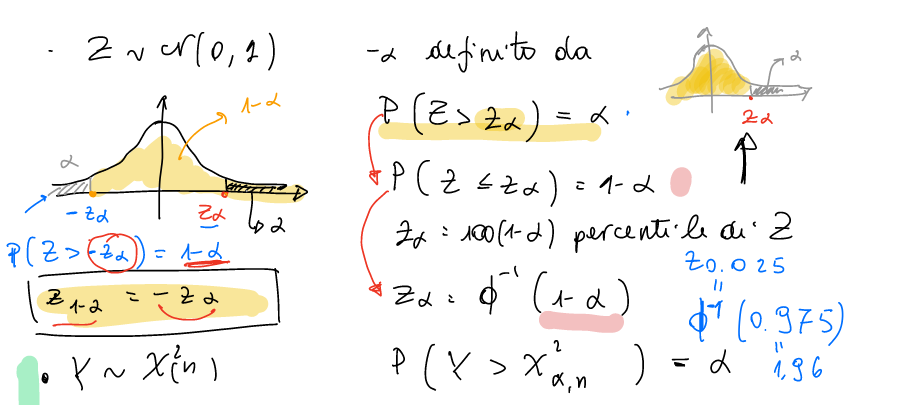
\includegraphics[width=120mm,scale=0.5]{Simmetria t di student.png}
\end{center}

\section{Stima per intervalli - Intervalli di confidenza}
Consideriamo la stima per intervalli della media di un campione normale $\mathcal{N}(\mu, \sigma^2)$, con
varianza $\sigma^2$ nota.
\\$\bar{X}_n$ è uno stimatore di $\mu$, e sappiamo che al crescere di $n$ la stima di $\mu$  più affidabile.
Vogliamo qunatificare questa affidabilità, construendo un intervallo \emph{centrato in $\bar{X}_n$} a cui $\mu$ appartenga con probabilità $\alpha$.
Si vuole cercare l'ampiezza $E$ di questo intervallo:
\[ P(|\bar{X}_n - \mu| < E) = 1-\alpha \to ... \to 
P(\mu \in (\bar{X}_n - \frac{z_\alpha}{2} \cdot \frac{\sigma}{\sqrt{n}},\bar{X}_n + \frac{z_\alpha}{2} \cdot \frac{\sigma}{\sqrt{n}}) )
\]
L'intervallo $(\bar{X}_n - \frac{z_\alpha}{2} \cdot \frac{\sigma}{\sqrt{n}},\bar{X}_n + \frac{z_\alpha}{2} \cdot \frac{\sigma}{\sqrt{n}})$
è l'intervallo di confidenza per $\mu$ di livello $100(1-\alpha)\%$.
\\Prima di eseguire le osservazioni questo è un intervallo aleatorio, quindi i suoi estremi sono V.A. e allora ha senso parlare di Probabilità
che il valore edl parametro $\mu$ appartenga a questo intervallo.
\\ Eseguite le osservazioni si ottiene un itervallo numerico a cui il valore del paramtreo $\mu$ appartiene con una confidenza del $100(1-\alpha)\%$.
Questo intervallo è simmetrico rispetto a $\bar{x}_n$.
\osservazione{ $E$, ovvero l'ampiezza dell'intervallo, rappresenta l'errore che commetto stimando $\mu$ con $\bar{x}_n$. }

\paragraph{Bontà della stima}
Ricordando che $E$ rappresenta l'errore che commetto stimando $\mu$, 
la bontà della stima dipende da:
\begin{itemize}
    \item Livello di confidenza: maggiore è il livello, più è affidabile è la stima ma più aumenta l'ampiezza.
    \item Ampiezza dell'intervallo = $2E$: più è piccolo, più è precisa la stima
\end{itemize}
\[
    E=Z_{\frac{\alpha}{2}}\frac{\sigma}{\sqrt{n}}
\]


$E$ cresce se $\alpha$ diminuisce (ossia se la confidenza aumenta) fissati $n$ e $\sigma$
$E$ diminuisce al crescere di n (come $\frac{1}{\sqrt[]{n}})$, fissati $\alpha$ e $\sigma$



\subsection[Estremi Inferiori e Superiori di Confidenza]{Estremi Inferiori e Superiori di Confidenza Per la media di una popolazione normale con varianza nota.}
Per determinare se la media di una popolazione è maggiore o minore di un certo
valore, uso gli estremi inferiori e superiori.
\\ Useremo ancora $\frac{\bar{X}_n - \mu}{\frac{\sigma}{\sqrt[]{n}}} = 
\sqrt[]{n} \frac{\bar{X}_n - \mu}{\sigma} \sim \mathcal{N}(0,1)$ 
\\ Confidenza: $100(1-\alpha) \%$
\begin{gather*}
    \mathbb{P}(\frac{(\bar{X}_n - \mu)}{\frac{\sigma}{\sqrt[]{n}}} < z_\alpha) 
    = 1 - \alpha \\
    \mathbb{P}(\mu > \bar{X}_n - z_\alpha \frac{\sigma}{\sqrt[]{n}} = \ - \alpha)
\end{gather*}
Un estremo inferiore di confidenza al $100(1-\alpha)\%$ per la media di una
popolazione normale con varianza nota è dato da
\begin{equation*}
    \bar{X}_n - z_\alpha \frac{\sigma}{\sqrt[]{n}}
\end{equation*}
La sua realizzazione (dai dati campionari) è:
\begin{equation*}
    \bar{x}_n - z_\alpha\frac{\sigma}{\sqrt[]{n}}
\end{equation*}
\subsection*{Intervalli di confidenza per la media di una popolazione normale con varianza incognita}
Completare -----------------------------------
Possiamo dire:
\begin{itemize}
    \item Confidenza maggiore $\rightarrow$ E aumenta (a parità del campione), però la
    stima è più affidabile
    \item Estremo inferiore di confidenza al $100(1-\alpha) \%$
    \item Estremo superiore di confidenza al $100(1-\alpha) \%$
\end{itemize}
\subsection*{Intervalli di confidenza per la varianza di una popolazione normale}

%Verifica di Ipotesi%
